\section{Power Supply}
This section will explain in detail the design of the power supply that was created to drive the various parts of the brick sorter. Three rails will be created, two using linear voltage regulators and one using a switching regulator. The power supply will be tested to verify that it conforms with the given performance requirements.
\subsection{Parts and Requirements}
The power supply described in this section is to have three voltage rails:
\begin{itemize}
	\item LEDs: 12v/1000mA.
	\item SERVO: 6v/1500mA.
	\item FPGA: 5v/1A, $\pm$\% max output voltage, min 80\% efficient.
\end{itemize}
The power supply itself is supplied with 15v. A list of components was provided in order to facilitate the design process. These are the main components of the power supply:
\begin{itemize}
	\item LM2574: Step-Down Switching Regulator. Datasheet \cite{lm2574}
	\item NCP7812TG: 12v Linear Voltage Regulator. Datasheet \cite{ncp7812}
	\item L7806cv: 6v Linear Voltage Regulator. Datasheet \cite{l7806}
\end{itemize}
Additionally, a PCB must be designed for the power supply.
\subsection{Design}
Since most of the components of the power supply are given, the task of design is mostly one of laying out the PCB. This is done by using Eagle\footnote{CadSoft EAGLE v7.4.0 Light Edition}. The schematics of the three different voltage rails can be seen in figure \ref{fig:psuschematic}.
The capacitors $C_3$ and $C_5$ are dimensioned according to the application circuit from their respective datasheet. They are omittable at low current operation or if the regulator is an appreciable distance from its power source. With no way of interpreting "appreciable distance" and operation being 1A and 1.5A for the 12v rail and the 6v rail respectively, it was decided to include them. Likewise, capacitors $C_4$ and $C_6$ serve to improve the transient response of the component.

The output and input of the linear voltage regulators is connected using a flyback diode. This is especially important on the 6V rail. This rail will be connected to the servomotor which, in a sense, is a coil, which can produce significant back electromotive force that could potentially damage the circuit.

The inherent inefficiency of linear voltage regulators gives cause to some thermal considerations, as any excess voltage is converted to heat. According to the datasheet, the NCP7812 has a junction-to-case thermal resistance $R_{\theta\text{JC}}=7.5^\circ\text{C/W}$. For the L7806, $R_{\theta\text{JC}}=5^\circ\text{C/W}$ See table \ref{tab:thermals} for an overview of the theoretical maximum operating temperature, $T_\text{max}$ with no heatsink. As can be seen the 12V rail would reach a maximum of 90$^\circ$C which is well below the maximum junction temperature of 125$^\circ$C listed in the datasheet, but well above what is considered pleasant to touch. To avoid burns while testing a heatsink is mounted. The 6V rail should not require a heatsink.

\begin{table}[h!]
	\centering
	\begin{tabular}{| c | c | c | c |}
		\hline
		Rail & Max curr. [A] & Max pow. [W] & $T_\text{max}$ [$^\circ$C] \\
		\hline
		12V  & 1.0 & 12 & 90 \\
		\hline
		6V   & 1.5 & 9 & 45\\
		\hline		
	\end{tabular}
	\caption[Maximum operating temperature]{Calculated maximum operating temperature of the 6V and 12V rails.}
	\label{tab:thermals}
\end{table}

\begin{figure}[h!]
	\begin{subfigure}{.48\linewidth}
		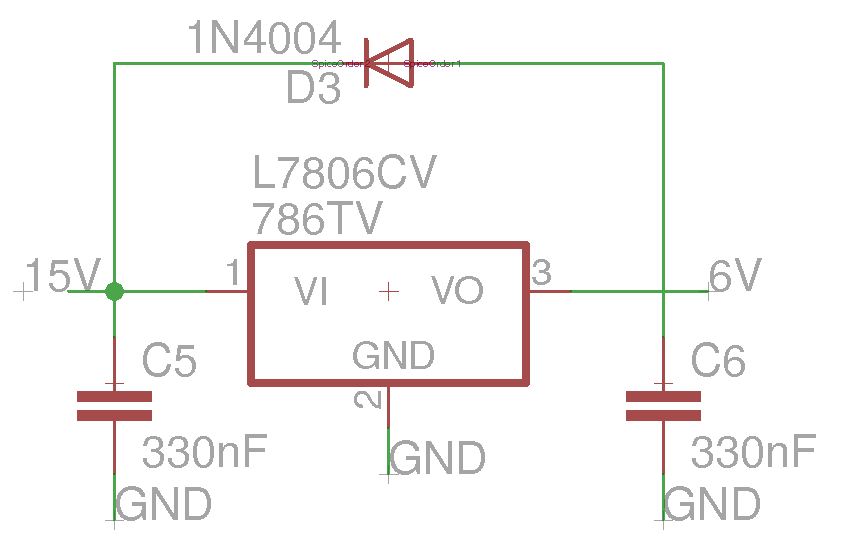
\includegraphics[width=\linewidth]{images/linear6v}
		\caption{Circuit for 6v rail.}
		\label{fig:psu6v}
	\end{subfigure}
	\begin{subfigure}{.48\linewidth}
		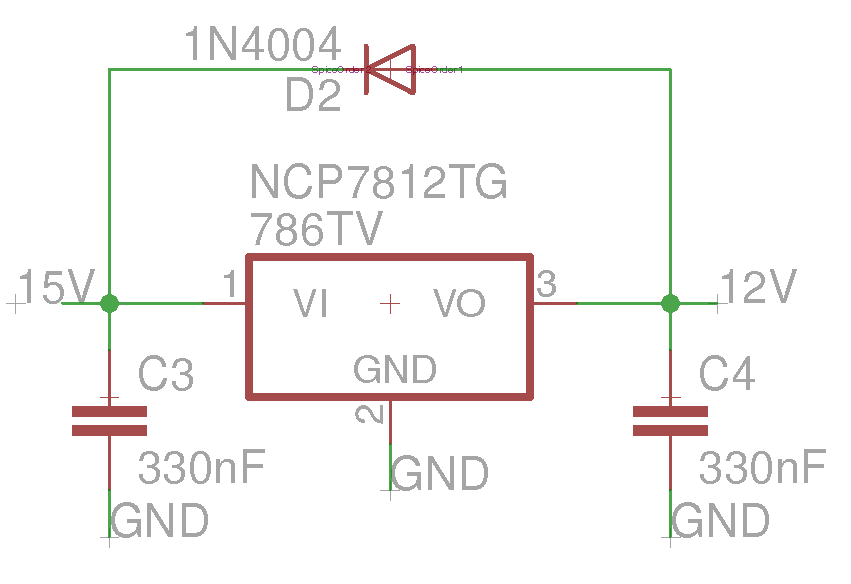
\includegraphics[width=\linewidth]{images/linear12v}
		\caption{Circuit for 12v rail.}
		\label{fig:psu12v}
	\end{subfigure}\\
	\begin{subfigure}{\linewidth}
		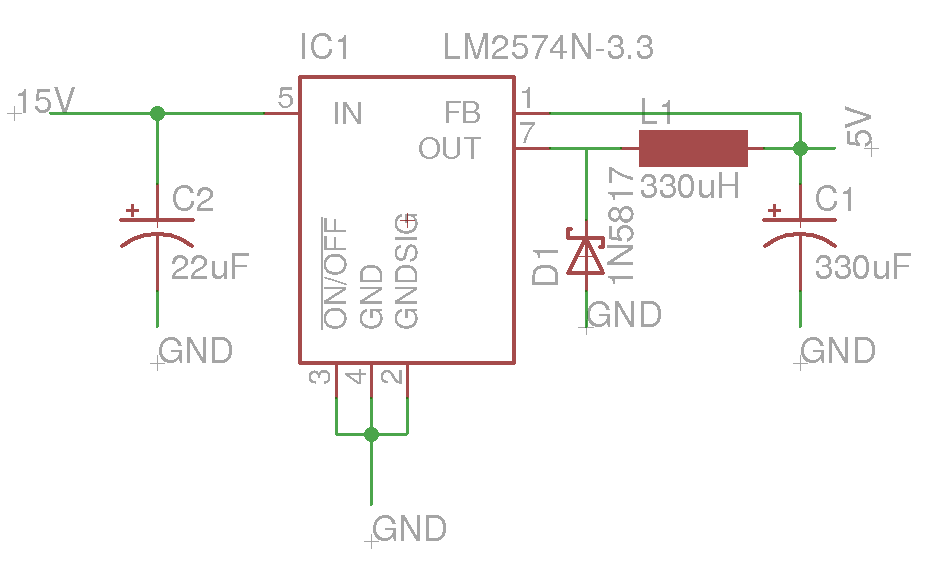
\includegraphics[width=\linewidth]{images/switch5v}
		\caption{Circuit for 5v rail.}
		\label{fig:psu5v}
	\end{subfigure}
	\caption{Schematics of the power supply.}
	\label{fig:psuschematic}
\end{figure}

The switching regulator in figure \ref{fig:psu5v} is designed as the typical applications design in the datasheet of the LM2574 \cite{lm2574}. This design is accompanied with a graph for dimensioning the size of the output inductance, $L_1$, see figure \ref{fig:inductorselect}. Since the IC will be supplied with 15V and a maximum load of 0.5A is required, the inductor necessary is 330$\mu$H. The value of the output capacitor, $C_1$ is determined according to 
\begin{eqnarray}
	C_\text{out}\geq&13300\frac{V_\text{in}(\text{MAX})}{V_\text{out}\cdot L(\mu\text{H})}(\mu\text{F})\\
	C_\text{out}\geq&13300\frac{15}{5\cdot 330} = 120.9(\mu\text{F})
\end{eqnarray} 
For this design, a 330$\mu$F capacitor is provided, which, while large, does fulfil the specification.
\begin{figure}[h!]
	\centering
	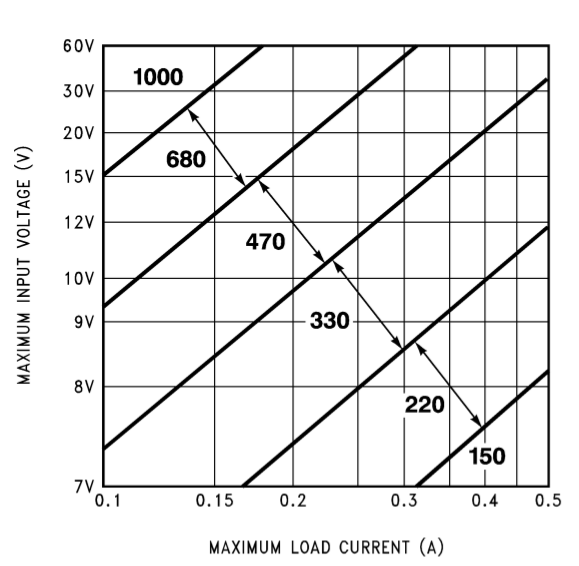
\includegraphics[width=.6\linewidth]{images/inductorselector}
	\caption{Graph showing the necessary inductance at various voltages and loads.}
	\label{fig:inductorselect}
\end{figure}
\\~\\

\subsection{Testing}
As previously mentioned the 5V rail must be at least 80\% efficient. However, according to the datasheet, the 5V version of the LM2574 is capable only of 77\% efficiency. Even though achieving the goal of 80\% efficiency will be difficult, the efficiency of this rail, as well as the others can still be tested and documented. Each rail will be tested for efficiency at 25\%, 50\%, 75\% and 100\% load. The results of this test can be seen in table \ref{tab:efficiency}. 
\begin{table}[h!]
	\centering
	\begin{tabular}{| c | c | c | c | c |}
		\hline
		Rail & Eff. 25\% & Eff. 50\% & Eff. 75\% & Eff. 100\% \\
		\hline
		12V  & 74.04 & 76.86 & 77.89 & 78.43\\
		\hline
		6V   & 37.89 & 38.95 & 39.31 & 39.45\\
		\hline		
		5V   & 75.75 & 76.19 & 76.34 & 77.24\\
		\hline
	\end{tabular}
	\caption[Power supply efficiency]{Efficiency of the various rails on the power supply.}
	\label{tab:efficiency}
\end{table}
As expected, the 5v rail peaks at $\approx77\%$ efficiency. The two rails controlled by linear voltage regulators clearly show the deficiencies of this technology. In the case of the 12V rail efficiency seems good, however it turns out that this efficiency is approximately equal to the relation between the input and output of the regulator, the same as for the 6V rail. The higher the difference between the input and output rails, the worse the efficiency. 